% Licensed to the Apache Software Foundation (ASF) under one or more
% contributor license agreements. See the NOTICE file distributed with
% this work for additional information regarding copyright ownership.
% The ASF licenses this file to You under the Apache License, Version 2.0
% (the ``License''); you may not use this file except in compliance with
% the License. You may obtain a copy of the License at
%
% http://www.apache.org/licenses/LICENSE-2.0
%
% Unless required by applicable law or agreed to in writing, software
% distributed under the License is distributed on an ``AS IS'' BASIS,
% WITHOUT WARRANTIES OR CONDITIONS OF ANY KIND, either express or implied.
% See the License for the specific language governing permissions and
% limitations under the License.

\subsubsection{Configuring a FileNet Connector}

You must fill in the following tabs if you are configuring a
FileNet Connector:

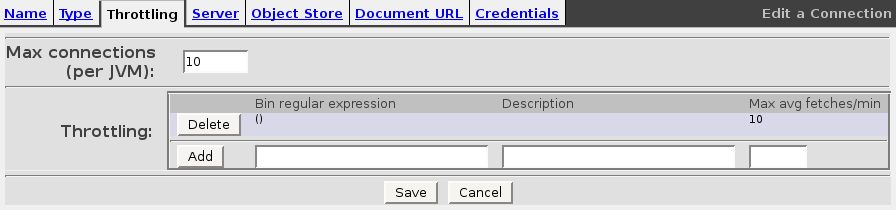
\includegraphics[width=300pt]{fln-edit-repository-tab3}

\begin{itemize}

\item \textbf{Max connections (per JVM):} Here you can set the maximum
number of connections to your repository.  \ifCombinedConnectorGuide
The maximum number of connections per JVM is important for three
reasons; licensing, appliance resources, and the possiblity of
overwhelming the ingestion interface. For a more complete explanation,
see the Max Connections item on page \pageref{maxrepocon}.\fi

\ifJDBCGuide
The maximum number of connections per JVM is important for several
reasons.  First, the number of connections may impact licensing and
available resources on your FileNet server.

Second, the number of connections may impact the resources available
on the appliance. If the connector framework is slowing down your
appliance, lowering this number should help.

Third, only ten document streams can be processed by the appliance
at one time.  If you are also using other repository connectors or
the \command{ingest} command on the appliance, you should reduce this
number to prevent contention for the Ingestion interface. The FileNet 
Connector will never overwhelm the interface on its own, but when other
applications are also using the ingestion interface, it may be best to
set the number of repository connections to five or even fewer.
\fi


\item \textbf{Throttling:} Here you can set a maximum document fetch
rate for the repository connection.  The maximum fetch rate allows you
to set three things: Expression, description, and fetches per minute.

In the FileNet Connector, the expression field can be used to create
throttle groups based on server name. Each FileNet Repository
Connection connects to only one server; use the blank match expression
\texttt{()} to match the server. Ask your FileNet administrator for an
appropriate limit on the number of fetches per minute. Enter the
information, and click Add.

\end{itemize}

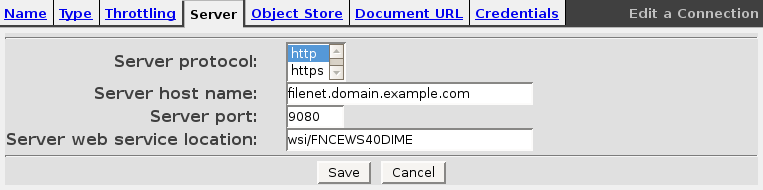
\includegraphics[width=300pt]{fln-edit-repository-tab4}

To fill out this tab, you will need information about the FileNet
service with which you wish to connect. You should ask your FileNet
administrator for this information.

\begin{itemize}

\item \textbf{Server protocol:} Select ``http'' or ``https'' using the drop down box. 

\item \textbf{Server host name:} The host name (including domain information) of your FileNet server.

\item \textbf{Server port:} The port to use to connect to the server. You should ask your FileNet administrator for the correct port.

\item \textbf{Server web service location:} The location of the FileNet web service on the server specified above.

\end{itemize}

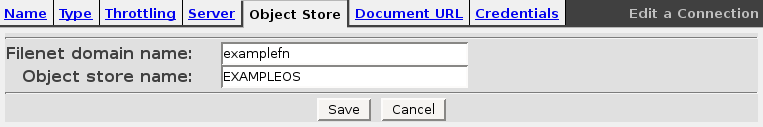
\includegraphics[width=300pt]{fln-edit-repository-tab5}

On this tab you will need to enter the FileNet domain name and object
store name. You will need to ask your FileNet administrator for this
information.

\begin{itemize}

\item \textbf{Filenet domain name:} The FileNet domain for the FileNet services. This is \textbf{not} the same as the Active Directory domain that your FileNet server is joined to.

\item \textbf{Object store name:} The name of the object store that you wish to crawl.

\end{itemize}

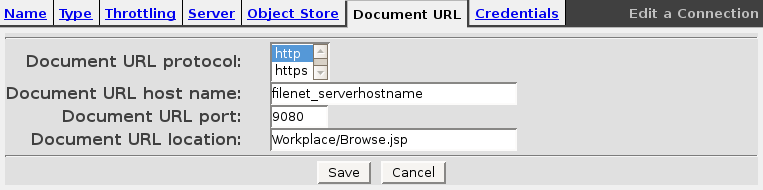
\includegraphics[width=300pt]{fln-edit-repository-tab6}

The information that you provide on this tab will be used to create
document URLs for the crawled documents. You should ask your FileNet
administrator for the information for your FileNet Access Engine.

\begin{itemize}

\item \textbf{Document URL protocol:} Select ``http'' or ``https'' using the drop down box. 

\item \textbf{Document URL host name:} The hostname of the Access Engine server.

\item \textbf{Document URL port:} The port to use to connect to the FileNet Access Engine server.

\item \textbf{Document URL location:} The location of the FileNet Access Engine service.

\end{itemize}

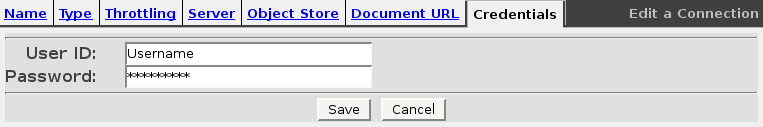
\includegraphics[width=300pt]{fln-edit-repository-tab7}

\item \textbf{User name:} This should be the user name used by your MetaCarta appliance, typically an Active Domain user name in the format \texttt{domain$\backslash$username}.

\item \textbf{Password:} The password corresponding to the user name given.



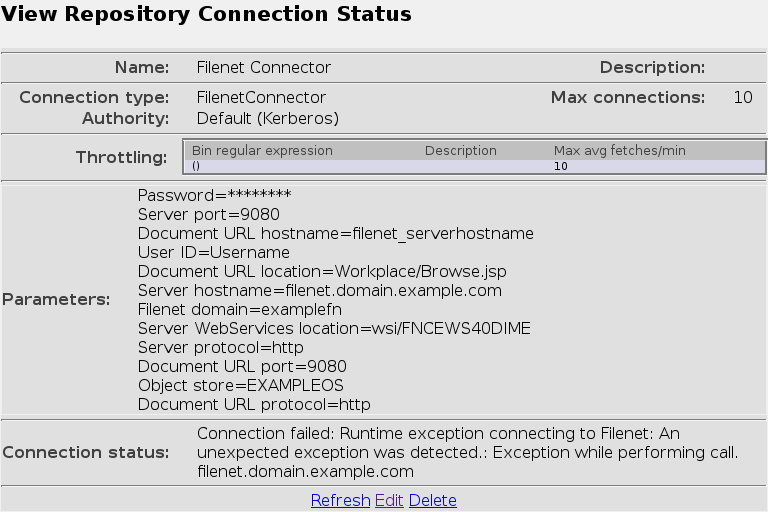
\includegraphics[width=300pt]{fln-view-repo-conn-status}

In this example (which does not contain accurate information for any
FileNet Connector), the Connection Status is ``Connection failed.''
If connetion has failed, the status message may contain information about
the failure.  If you see an error message, the FileNet server might be
down, or you might have incorrectly entered data into one of the fields,
If so, you should click ``Edit'' to fix the data. If you have entered
everything as you intended, please inform your database administrator;
you may not have been given the correct information.
